\begin{adjustbox}{width=\textwidth}
	\begin{tikzpicture}[every node/.style={inner sep=0,outer sep=0}]
	
		\node [anchor=north east] (imgSpalten) at (-0.03\textwidth,0) {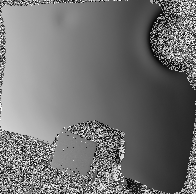
\includegraphics[width=.47\textwidth]{04_deflektometrischeRegistrierung/auswertungDeflektometrischeRegistrierung/figures/spaltenRegistrierung_Delle}};
		\node [below=0.2cm of imgSpalten] {Graubild der Spaltenzuordnung \acrshort{frx}$(x,y)$};
		\node [anchor=north west] (imgZeilen) at (0.03\textwidth,0) {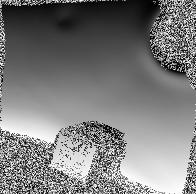
\includegraphics[width=.47\textwidth]{04_deflektometrischeRegistrierung/auswertungDeflektometrischeRegistrierung/figures/zeilenRegistrierung_Delle}};
		\node [below=0.2cm of imgZeilen] {Graubild der Zeilenzuordnung \acrshort{fry}$(x,y)$};
		
	\end{tikzpicture}
\end{adjustbox}
\caption[Deflektometrische Registrierung bei Delle]{Deflektometrische Registrierung des spiegelnden Keramikobjekts aus Abbildung \ref{img:objektMitDelle}.}